\anhang{Umfrage Kriterienpriorisierung}\label{anhang:umfrage}
Mithilfe des Tools Questionpro wurde eine Umfrage erstellt, um Architekten der SPIRIT/21 GmbH im Bereich Native Cloud die Möglichkeit zu geben, die Kriterien für die Produkt/Dienslteistungsbewertung via \enquote{Drag \& Drop} selber zu priorisieren.

Die Umfrage präsentierte sich folgendermaßen:

\begin{figure}[H]
\centering
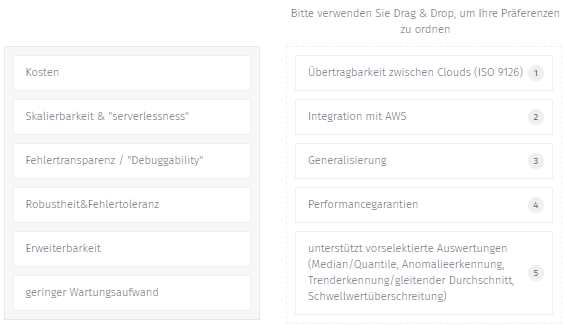
\includegraphics[width=\textwidth]{graphics/Umfrage-Darstellung.png}
\caption{Die Umfrage in QuestionPro}
\label{abb:Umfrage}
\end{figure}


\begin{table}[H]
\centering
\begin{tabular}{|l|l|}
\hline
Kriterium & Average \\ \hline
Übertragbarkeit zwischen Clouds (ISO 9126) & 1,00 \\ \hline
Integration mit AWS & 2,00 \\ \hline
Generalisierung & 3,00 \\ \hline
Erweiterbarkeit & 4,67 \\ \hline
Fehlertransparenz / \enquote{Debuggability} & 5,67 \\ \hline
geringer Wartungsaufwand & 6,67 \\ \hline
Kosten & 7,33 \\ \hline
Skalierbarkeit  \& \enquote{serverlessness} & 7,33 \\ \hline
Robustheit \& Fehlertoleranz & 9,67 \\ \hline
Performancegarantien & 8,33 \\ \hline
unterstützt Auswertungen (\autoref{chap:auswertungsarten}) & 10,33 \\ \hline
\end{tabular}
\caption{Auswertungen der Umfragen}
\label{tab:umfragen-auswertungen}
\end{table}

Insgesamt nahmen $n=3$ Personen teil. Die Ergebnisse sind in \autoref{tab:umfragen-auswertungen} dargestellt.